\documentclass[border=5pt]{standalone}
\usepackage{xcolor}
\usepackage{pgfplots}
\usepackage{tikz}
\usetikzlibrary{patterns}
% Define bar chart colors
%
\definecolor{bblue}{HTML}{4F81BD}
\definecolor{rred}{HTML}{C0504D}
\definecolor{ggreen}{HTML}{9BBB59}
\definecolor{ppurple}{HTML}{9F4C7C}
\definecolor{orange}{HTML}{FF7E00}
\definecolor{yellow}{HTML}{FFFF66}

\pgfplotsset{every tick label/.append style={font=\large}}

\begin{document}
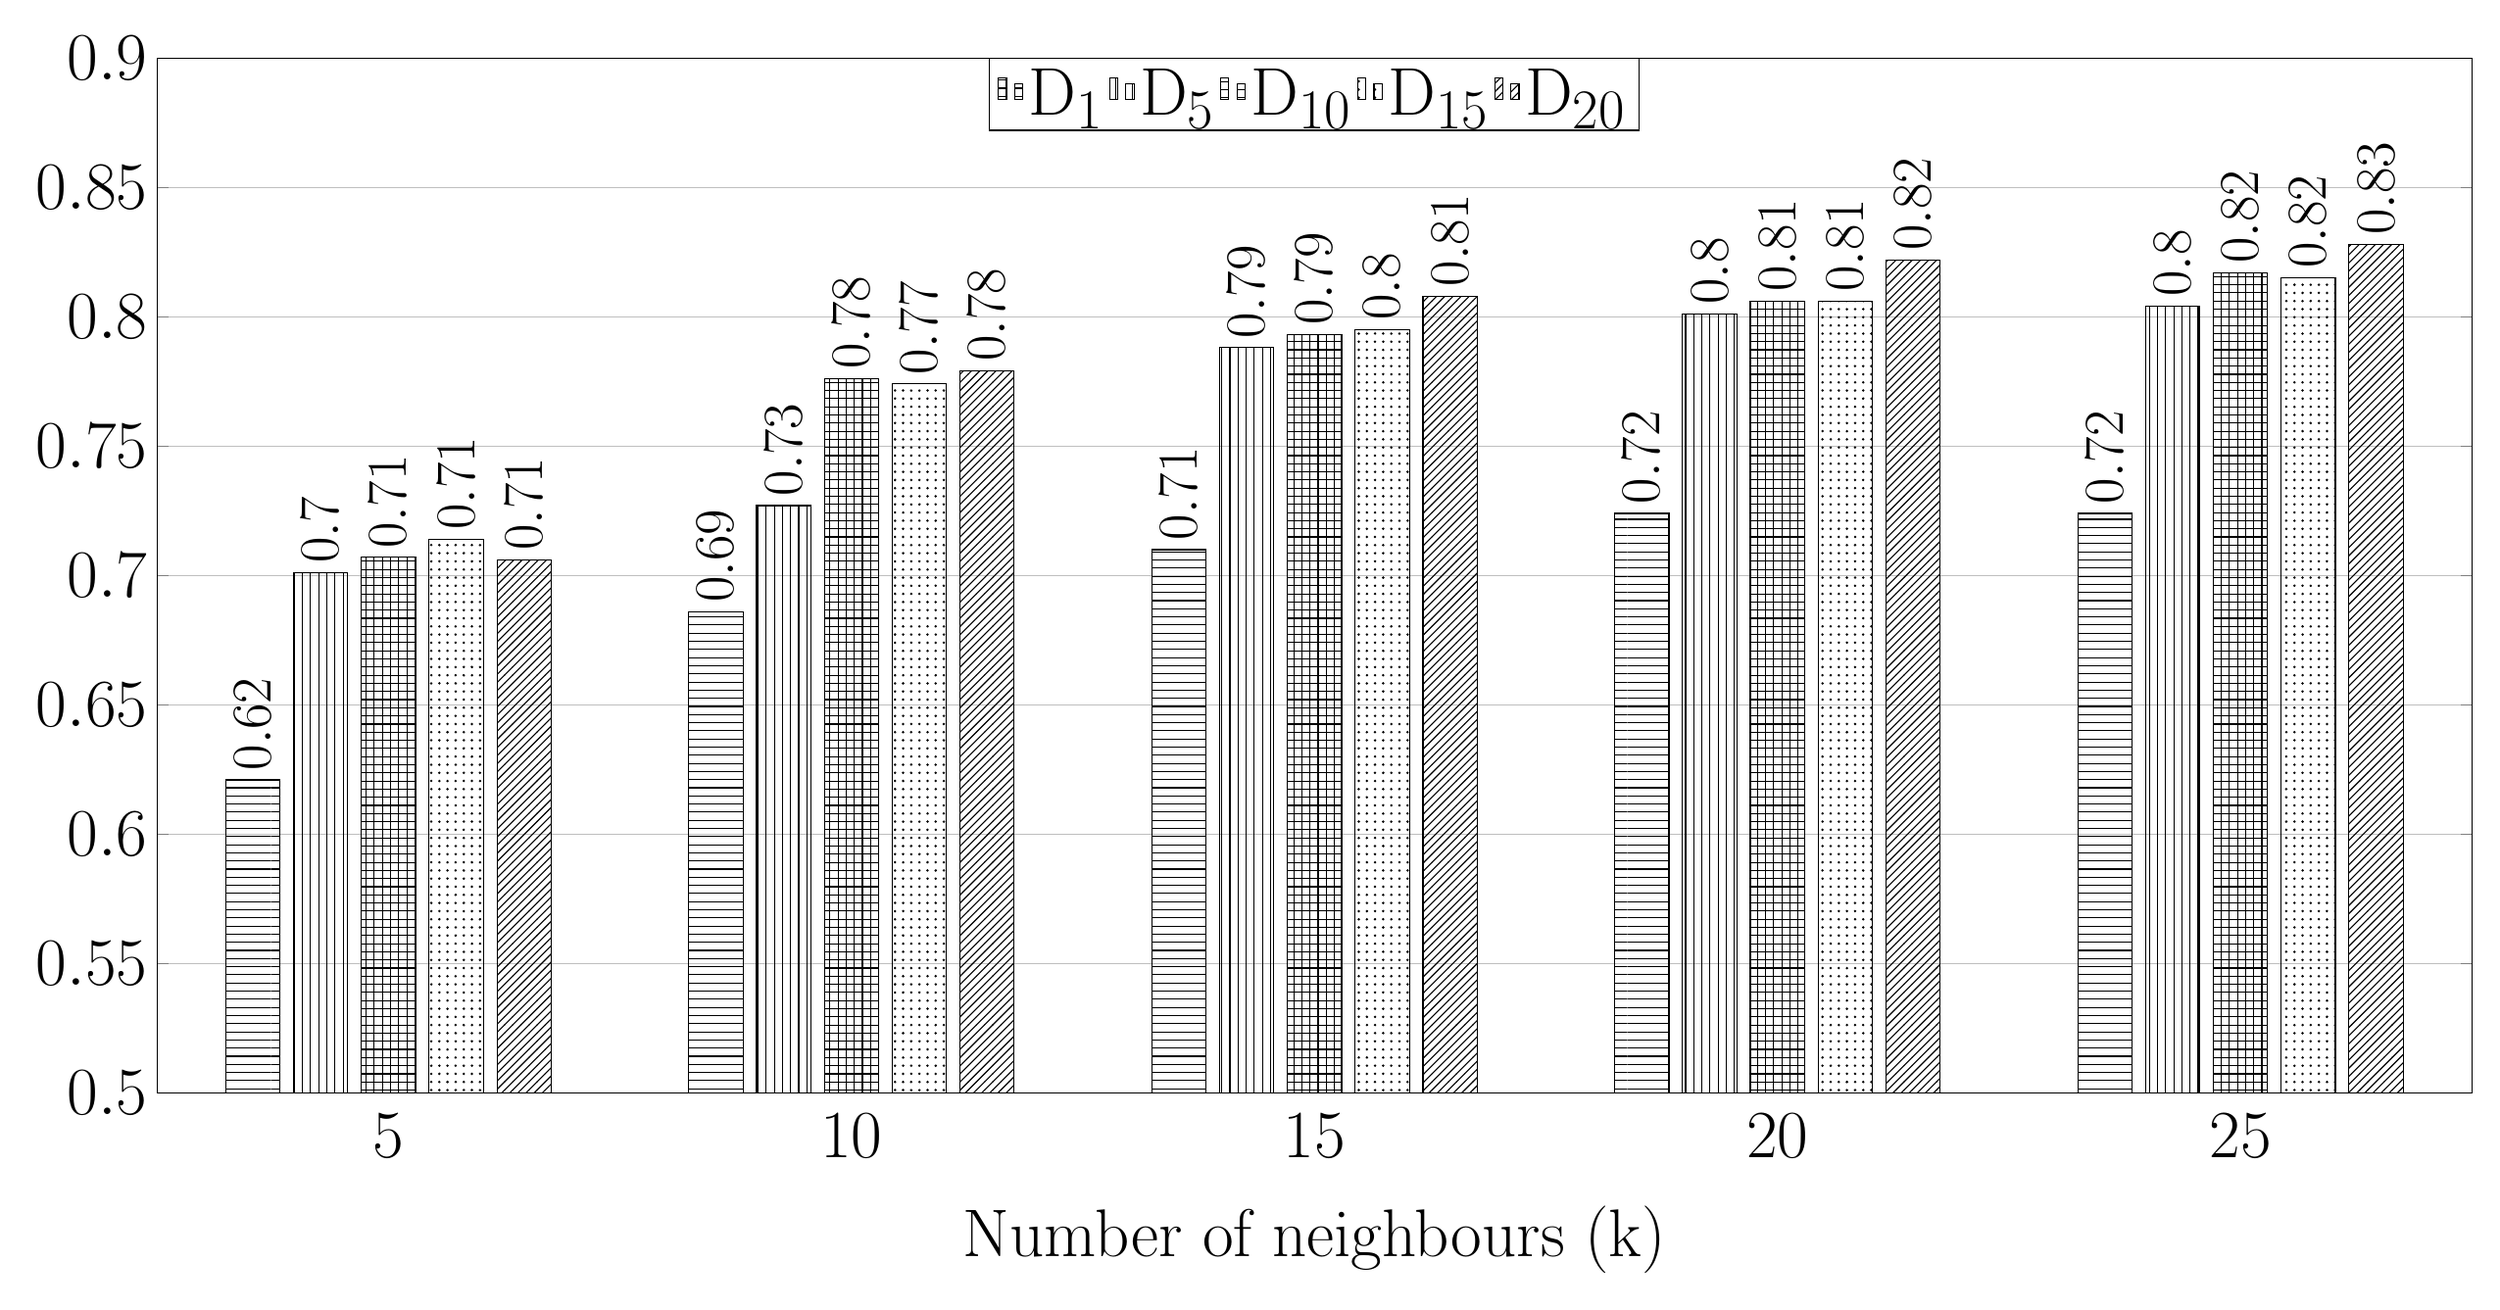
\begin{tikzpicture}
    \begin{axis}[
        width  = 6cm,%*\textwidth,
        height = 15	cm,
        major x tick style = transparent,
        ybar = 5pt,
        ymin = 0.5, ymax = 0.9,
        x=6cm,
        bar width=20pt,
        ymajorgrids = true,	
        xtick = data,
        scaled y ticks = false,
%		legend style={at={(0.5,-0.1)},
%		legend style={at={(0.5,1.1)}, anchor=north,legend columns=-1,font=\small},
      	legend style={at={(0.5,1)},	anchor=north,legend columns=-1,font=\Huge,
		anchor=north,legend columns=-1},
		enlarge x limits={abs=3cm},
		nodes near coords,
		nodes near coords style={font=\huge},
		every node near coord/.append style={rotate=90, anchor=west},
	    xlabel={Number of neighbours (k)},
	    %ylabel = {Success rate@5 (\%)},
   	    xlabel style={font=\Huge, at={(axis description cs:0.5,-0.1)},},
	    every tick label/.append style={font=\Huge},
        symbolic x coords={5,10,15,20,25},
    ]
        \addplot[style={black,fill=blue!30,mark=none,pattern=horizontal lines}]
            coordinates {(5, .621) (10, 0.686) (15,0.710)(20, 0.724)(25, 0.724)};
            
		\addplot[style={black,fill=orange!30,mark=none, pattern=vertical lines}]
            coordinates {(5, 0.701) (10, 0.727) (15,0.788)(20, 0.801)(25, 0.804)};
                      
        \addplot[style={black,fill=red!30,mark=none,pattern=grid}]
            coordinates {(5,0.707) (10,0.776) (15,0.793)(20,0.806)(25,0.817)};

        \addplot[style={black,fill=green!30,mark=none, pattern=dots}]
            coordinates {(5,0.714) (10,0.774) (15, 0.795) (20,0.806) (25,0.815)};

        \addplot[style={black,fill=purple!30,mark=none, pattern=north east lines}]
            coordinates {(5,0.706) (10,0.779) (15,0.808) (20,0.822) (25,0.828)};

        \legend{D$_1$, D$_5$, D$_{10}$, D$_{15}$, D$_{20}$}
    \end{axis}
\end{tikzpicture}
\end{document}